%%%%%%%%%%%%%%%%%%%%%%% file template.tex %%%%%%%%%%%%%%%%%%%%%%%%%
%
% This is a general template file for the LaTeX package SVJour3
% for Springer journals.          Springer Heidelberg 2010/09/16
%
% Copy it to a new file with a new name and use it as the basis
% for your article. Delete % signs as needed.
%
% This template includes a few options for different layouts and
% content for various journals. Please consult a previous issue of
% your journal as needed.
%
%%%%%%%%%%%%%%%%%%%%%%%%%%%%%%%%%%%%%%%%%%%%%%%%%%%%%%%%%%%%%%%%%%%
%
\RequirePackage{fix-cm}
%
%\documentclass{svjour3}                     % onecolumn (standard format)
\documentclass[smallcondensed]{svjour3}     % onecolumn (ditto)
%\documentclass[smallextended]{svjour3}      % onecolumn (second format)
%\documentclass[twocolumn]{svjour3}          % twocolumn
%
\smartqed  % flush right qed marks, e.g. at end of proof
%
\usepackage{graphicx}
%
% \usepackage{mathptmx}      % use Times fonts if available on your TeX system
%
% insert here the call for the packages your document requires
%\usepackage{latexsym}
% etc.
%
% please place your own definitions here and don't use \def but
% \newcommand{}{}
%
% Insert the name of "your journal" with
\journalname{AStA Advances in Statistical Analysis}

% Own Packages and newcommands
\usepackage{amsmath, amssymb}
\usepackage{bm}
\setlength{\parindent}{0pt} % remove indentation before every paragraph
\usepackage{booktabs}
\usepackage{multirow}
\usepackage{float} % to force figure placement
\usepackage[usenames, dvipsnames]{color}
% \usepackage[backend=bibtex,
%             style=nature,
%             citestyle=authoryear]{biblatex}
% \addbibresource{bauer_2018.bib}
\usepackage{natbib}
\bibliographystyle{smj}
\newcommand{\T}{\mathrm{\scriptscriptstyle T}}
\newcommand{\red}[1]{\textcolor{red}{#1}}



\begin{document}
\title{KOALA: A new paradigm for election coverage %\thanks{Grants or other notes
%about the article that should go on the front page should be
%placed here. General acknowledgments should be placed at the end of the article.}
}
\subtitle{A opinion poll based "now-cast" of event probabilities in multi-party electoral systems}
\titlerunning{KOALA: Coalition analyses}   % if too long for running head

\author{Alexander Bauer \and Andreas Bender \and Andr\'e Klima \and Helmut K\"{u}chenhoff}

%\authorrunning{Short form of author list} % if too long for running head

\institute{A. Bauer \at
              Statistical Consulting Unit StaBLab, Department of Statistics, LMU Munich, Germany \\
              Tel.: +49-89-2180-3197 \\
              Fax: +49-89-2180-5308 \\
              \email{alexander.bauer@stat.uni-muenchen.de} \\
              ORCID: 0000-0003-3495-5131
%             \emph{Present address:} of F. Author  %  if needed
           \and
           A. Bender \at
              Statistical Consulting Unit StaBLab, Department of Statistics, LMU Munich, Germany \\
              ORCID: 0000-0001-5628-8611
           \and
           A. Klima \at
              Statistical Consulting Unit StaBLab, Department of Statistics, LMU Munich, Germany
           \and
           H. K\"{u}chenhoff \at
              Statistical Consulting Unit StaBLab, Department of Statistics, LMU Munich, Germany
}

\date{Received: date / Accepted: date}
% The correct dates will be entered by the editor


\maketitle

\begin{abstract} \red{150 to 250 words} \\
Common election poll reporting is often misleading as sample uncertainty is
insufficiently addressed or  not covered at all. Furthermore, the main interest
is beyond the simple percentages of the contenders. For a more comprehensive
coverage, we propose shifting the focus towards reporting survey-based probabilities
of specific election outcomes. We present such an approach for multi-party
electoral systems, focusing on probabilities of coalition majorities.
A Monte Carlo based Bayesian Multinomial-Dirichlet model is used for estimation.
The method utilizes published opinion polls conducted by established polling
agencies and is accompanied by a pooling approach to summarize multiple current
surveys to reduce sample uncertainty, thereby accounting for dependencies between
polling agencies. Sample uncertainty-based probabilities are estimated, assuming
the election was held today, not accounting for potential shifts until election.
Since our method is based on the posterior distribution of the election outcome,
our method can be applied to specific questions relating to the outcome of the election.

Possible visualizations of the results are shown and the benefit of the approach is outlined
by discussing election polls before the German federal elections 2013 and 2017.
An implementation is freely available in the \texttt{R} package \texttt{coalitions}.

\keywords{\red{4 to 6 keywords} Election analysis \and Opinion polls \and Election reporting \and Multinomial-Dirichlet \and Pooling}
% \PACS{PACS code1 \and PACS code2 \and more}
% \subclass{MSC code1 \and MSC code2 \and more}
\end{abstract}

\section{Introduction} \label{intro}
In multi-party democracies, approval of the government's  and the opposition
parties' work is usually measured by public opinion polls continuously conducted
and published by various polling agencies. Reported quantities
usually include the share of respondents that would vote for the respective
political parties {\it if the election was held today} (party shares),
the number of overall respondents and -- often less prominent -- information
about sample uncertainty.\\

One party often does not obtain enough votes for a governance majority by itself,
thus, multiple parties form a so-called \emph{coalition} to jointly obtain the
necessary majority of seats in parliament.
The mainstream media usually reports the results of such surveys by focusing
on the voter shares while ignoring sample uncertainty. This is often misleading,
especially if the shares are used to infer the possibility of a majority for
a specific coalition. For example, in the prelude to the 2017 German election,
a coalition was oftentimes stated to ``lose'' its majority just because the joint
voter share dropped under 50\% from one opinion poll to the next \citep[cf.][]{umfrage_2017}.
Such interpretations are clearly inadequate as sample uncertainty
(and often redistribution of votes) is not taken into account. This is especially
problematic, when one or more parties are close to the country-specific threshold
of votes that has to be passed in order to enter the parliament. Such a case
occurred in the 2013 German election, when reported share of the Free Democratic
Party (FDP) was close to the 5\% hurdle (cf. Section \ref{ssec:intro-ex-fdp}).\\

% Additionally, the perception of
% the observed voter shares to be definite values that hold for the
% electorate can also lead to an -- to some extent -- unjustified criticism
% of general opinion polls if the final election result differs
% from the latest polls published before election day. One prominent example is
% XXX

Beyond ensuring proper reporting of sample uncertainties, in our opinion, the
focus in election poll reporting should in general be shifted away from the
observed party shares. Instead, election coverage should focus on the most relevant
question, i.e., how {\it probable} is a specific event or election outcome, given
the current political mood.
As probabilities combine both, the observed shares and sample uncertainty in one
number, they allow more precise as well as more adequate statements about specific
events that can be easier to communicate to the general public and are
less prone to misinterpretation.
Events usually of interest before an election are
\begin{itemize}
  \item  "Will a party obtain enough votes to enter the parliament (pass the minimal threshold)?"
  \item  "Will a party obtain the most (second most, third most, etc.) votes?"
  \item "Will a specific coalition obtain enough votes (joint majority) to form a governing coalition?"
\end{itemize}


In this article, we present our approach for election and coalition analysis
(in German: \textbf{Koal}itions-\textbf{A}nalyse (KOALA)) that estimates the
probability of such events and brings more value to opinion-poll-based election
coverage. It is important to note that we quantify the contemporary political mood
and the resulting event probabilities ("now-cast"), not taking into consideration
potential shifts until election day ("fore-cast"). Approaches for predicting
future election outcomes based on past information can e.g. be found in
\citet{graefe_2017} or \citet{norpoth_gschwend_2010}. A special focus is put on
multi-party electoral systems and the estimation of probabilities for (joint) majorities.
Probabilities are estimated by Monte Carlo simulations of election outcomes from the
Bayesian posterior distribution of party shares conditional on current observed
opinion poll data. Prior to the German general elections 2013 and 2017, results
based on (an earlier iteration of) our approach already entered mainstream media
reporting \citep[cf.][]{wahlistik_2013, gelitz_2017}.\\

All methods discussed in this article are implemented in \texttt{R} \citep{r_2017}
and are available in the open-source package \texttt{coalitions} \citep{bender_bauer_2018}.
An interactive \texttt{shiny}-based \citep{chang_2017} website
\texttt{koala.stat.uni-\allowbreak muenchen.\allowbreak de} visualizes estimated
coalition probabilities and is used to communicate the results for German general
and federal elections to the general public. Additionally, we applied our method
to the Austrian general election 2017. The process of fetching new polls,
updating the website and sending out Twitter messages based on the newest results
is automated and allows for an immediate transfer of the estimated event
probabilities to media outlets as well as the general public.

\subsection{Data basis}\label{ssec:data-basis}
As database for our calculations, we use opinion polls conducted by established
polling agencies that quantify the electoral mood in a limited time-frame
(\textit{if an election was held today}). For each of the two elections discussed
in Section \ref{sec:application}, we base the discussion on opinion polls published
by major German polling agencies (i.e., Allensbach, Emnid, Forsa, Forschungsgruppe Wahlen,
GMS, Infratest dimap and INSA), starting one year before each election.
Opinion poll data from these polling agencies is publicly available
on \texttt{www.wahlrecht.de}. Application of our approach to other countries
requires systematic access to respective polling data. For the Austrian general
election in 2017 for example, we used the data base available at
\texttt{https://neuwal.com/wahlumfragen/}.


\subsection{A motivating example}\label{ssec:intro-ex-fdp}
In the last opinion poll conducted before the German federal election 2013 \citep{forsa_2013},
special interest was on whether the conservative ``Union'' -- i.e., a union of
the parties CDU and CSU -- and the liberal FDP would together obtain enough votes
to form the governing coalition (cf. Table \ref{tab_fdp}).

\begin{table}[!ht]\centering
\caption{Reported voter shares in the Forsa opinion poll for the German general
election, published September 20th, 2013 with $n=1995$ respondents.
\label{tab_fdp}
}
\medskip
\begin{tabular}{cccccccc}
\toprule[0.09 em]
Union & SPD & Greens & FDP & The Left & Pirates & AfD & Others \\
\midrule
40\% & 26\% & 10\% & 5\% & 9\% & 2\% & 4\% & 4\% \\
\bottomrule[0.09 em]
\end{tabular}
\end{table}

The German election system mandates a 5\% vote share for parties to enter the parliament.
Votes for parties below this threshold are redistributed (proportionally) to parties
above it. Table \ref{tab_fdp_redist} depicts the resulting redistributed voter
shares given the poll in Table \ref{tab_fdp}. It illustrates, that Union-FDP with
its 45\% voter share before redistribution, would obtain 50\% of parliament
seats after redistribution. Thus, ignoring uncertainty one would conclude that a
majority is possible for the coalition, if voter shares improve slightly for one
of the two parties.

\begin{table}[!ht]\centering
\caption{Redistributed voter shares based on the Forsa opinion poll for the German general election,
published September 20th, 2013 with $n=1995$ respondents (cf. Table \ref{tab_fdp}).
Party shares marked with ''--'' indicate parties that would not pass the 5\% hurdle.
\label{tab_fdp_redist}
}
\medskip
\begin{tabular}{cccccccc}
\toprule[0.09 em]
Union & SPD & Greens & FDP & The Left & Pirates & AfD & Others \\
\midrule
44.44\% & 28.89\% & 11.11\% & 5.56\% & 10.00\% & -- & -- & -- \\
\bottomrule[0.09 em]
\end{tabular}
\end{table}

However, such considerations completely ignore the sample uncertainty and the
probabilistic nature of the outcome. If the poll in Table \ref{tab_fdp} is representative,
one would expect that the FDP enters the parliament (passes the 5\% hurdle) with a
probability of about $50\%$. Thus, the (posterior) distribution of the joint voter
share is bimodal and also depends on whether the other "small" parties close to
the 5\% threshold enter the parliament. This example also illustrates that discussion
of reported party shares can become very complex, due to sample uncertainty
and the multitude of different outcomes this uncertainty entails.
We therefore argue that probability based reporting of opinion poll results can
answer the actual question of interest ("Will a coalition of Union-FDP obtain
enough votes to obtain a majority of seats in the parliament?") more directly, while
adequately taking into account the inherent uncertainty.\\

The remainder of the article is structured as follows: Section \ref{sec:methods}
introduces the Bayesian method used to estimate event probabilities as well
as some details on the aggregation of multiple opinion polls and the correction
of rounding errors. Section \ref{sec:application} illustrates the
application of the approach to opinion polls in advance of the  2013 and 2017
German general elections. A summary and discussion are presented in Section
\ref{sec:conclusion}.\\

\section{Methods}\label{sec:methods}
In this section, we describe our method for the estimation of event
probabilities based on reported party shares. Section~\ref{ssec:bayes} gives a
general introduction to the Multinomial-Dirichlet model. In Section~\ref{ssec:pooling}
our approach for the aggregation of multiple polls from different polling agencies
is described. As most agencies report rounded voter shares, we perform rounding
error adjustment, briefly discussed in Section~\ref{ssec:rounding}.

\subsection{Estimating event probabilities from reported voter shares} \label{ssec:bayes}
To estimate the probability of specific events conditional on opinion poll results
we use the Bayesian framework to construct the \emph{posterior} distribution of
the party shares based on distribution of the observed shares and an assumption
about their \emph{prior} distribution.\\

Let $X_1,\ldots, X_P$ the reported opinion poll count of respondents that would
elect party $X_p, p=1,\ldots,P$ (vote count). For example, in Table \ref{tab_fdp}
the reported vote count for the \emph{Union} is given by $X_1 = .40 \times 1995 = 798$.
Assuming that $(X_1, \ldots, X_P)$ has a Multinomial distribution
\begin{equation}\label{eq:multinom}
(X_1,\ldots, X_k) \sim Multinomial(n, \theta_1,\ldots, \theta_P),
\end{equation}

where $n$ is the sample size of the opinion poll and $\theta_p, p=1,\ldots,P$
indicates the probability of party $p$ being selected. Assuming a representative
random sample, $\theta_p$ represents the percentage of voters for party $p$ in
the general population (CITATION Stichproben Buch). Given one (pooled) survey,
the distribution of the observed vote counts $\mathbf{x}=x_1,\ldots,x_P$ is
denoted by $f(\mathbf{x}|\boldsymbol{\theta})$.\\

For the prior distribution of the true party shares $\boldsymbol{\theta}=\theta_1,\ldots, \theta_P$
we chose a flat, uninformative prior distribution
(Jeffrey's prior; \citet{gelman_2013})

\begin{equation}\label{eq:prior}
\begin{aligned}
\boldsymbol{\theta} &= (\theta_1,\ldots,\theta_P)^\T \sim Dirichlet(\alpha_1,\ldots,\alpha_P), \\
\text{with} &\ \ \ \ \ \ \ \ \ \ \ \ \ \ \ \alpha_1 = \ldots = \alpha_P = \frac{1}{2}
\end{aligned}
\end{equation}

and prior distribution $p(\boldsymbol{\theta}|\boldsymbol{\alpha})$.
As the Dirichlet distribution is a conjugate prior to the Multinomial distribution,
the resulting posterior distribution of parameters $\boldsymbol{\theta}|\mathbf{x}$

\begin{align}
f(\boldsymbol{\theta}|\mathbf{x})
  & = \frac{f(\mathbf{x}, \boldsymbol{\theta})}{f(x)}
    = \frac{f(\mathbf{x}|\boldsymbol{\theta})p(\boldsymbol{\theta}, \boldsymbol{\alpha})}{f(x)}\\
  & \propto f(\mathbf{x}|\boldsymbol{\theta})p(\boldsymbol{\theta}|\boldsymbol{\alpha})\\
  & \propto \prod_{p=1}^{P}\theta_p^{x_p}\cdot \prod_{p=1}^{P}\theta_p^{\alpha_{j}-1} = \prod_{p=1}^{P}\theta_p^{x_p + \alpha_p-1},
\end{align}

is again a Dirichlet distribution with
\begin{equation}\label{eq:posterior}
\boldsymbol{\theta}|\mathbf{x} \sim Dirichlet(x_1 + 1/2,\ldots, x_P + 1/2).
\end{equation}

Given the multivariate posterior \eqref{eq:posterior} and using Monte Carlo
simulations, probabilities for many types of events can be deduced by simulating
election outcomes from \eqref{eq:posterior} and calculating the percentage of
simulations in which the event of interest occurred. This includes the
probabilities for specific majorities derived from a complex, country-specific
system of rules for the calculation of seats in the parliament
(Sainte-Lague-Schepper in Germany; CITATION). For example, given the Forsa poll
introduced in Section \ref{ssec:intro-ex-fdp}, the coalition of Union-FDP
obtained a majority of seats in $2\,633$ of $10\,000$ simulations, which equals
an estimated probability of $26\%$ (see Section \ref{sec:application} for
more details).\\

If it is known that estimates of specific party shares are biased for some opinion
polls/agencies, this information could be included in the model by using an
informative prior distribution. The priory parameters $\alpha_p$ would than
be adjusted to have higher or lower values, respectively.
However, such biases of polling agencies are hard to quantify as the true party
share in the electorate is only known on election days. For our analyses, we
therefore use the uninformative prior \eqref{eq:prior}.

\subsection{Aggregation of multiple polls (Pooling)} \label{ssec:pooling}
In the presence of multiple published opinion polls, pooling is used to
aggregate multiple polls in order to reduce sample uncertainty.
To ensure a reliable pooling regarding the current public opinion,
we only use polls published within the past 14 days and only use the
most recent survey published by each polling agency.\\

Considering a single poll $i$, the observed number of votes $X_{ip}$ for each of
$P$ parties follow a multinomial distribution with sample size $n_i$ and underlying,
unknown party shares $\theta_p$ in the population.
% \begin{equation}
% X_{i1},\ldots, X_{ik} \sim Multinomial(n_i,\theta_1,\ldots,\theta_k).
% \end{equation}
Pooling over multiple such polls as independent random samples leads to another
multinomial distribution for the summed number of votes $\sum_i X_{ip}$:
% Based on the multinomial distribution of the vote counts $X_{ij}$ of party $j$ in poll $i$ with underlying true party share $\theta_j$, pooling over multiple polls representing independent random samples would lead to a multinomial distribution for the summed number of votes $\sum_i X_{ij}$:
\begin{equation}
\sum\limits_i X_{i1},\ldots, \sum\limits_i X_{iP}
  \sim Multinomial \left( \sum\limits_i n_i,\theta_1,\ldots,\theta_P\right).
\end{equation}

Further analyses, however, showed that polls from different (German)
polling agencies are correlated
and the independency assumption does not hold.
Therefore, we adjust the resulting multinomial
distribution by using an \textit{effective sample size} \citep{hanley_2003},
reflecting that the aggregation over multiple polls does not contain
information of a sample with $\sum_i n_i$ observations.\\

Quantification of pairwise correlation is done based on the variance of the
party share difference between two polls for a specific party.
The following equation holds for two independent
random sample polls $A$ and $B$:

\begin{equation}
\begin{aligned}
Var(X_A - X_B) &= Var(X_A) + Var(X_B) - 2 \cdot Cov(X_A, X_B) \\
\Leftrightarrow \ \ \ \ Cov(X_{Aj}, X_{Bj}) &= \frac{1}{2} \cdot \left(Var(X_{Aj}) + Var(X_{Bj}) - Var(X_{Aj} - X_{Bj}) \right).
\end{aligned}
\end{equation}

We take $Var(X_{Aj})$ and $Var(X_{Bj})$ as the theoretical variances of the binomially distributed, observed voter numbers and estimate $Var(X_{Aj} - X_{Bj})$ based on the observed differences between the party shares. Having done so, one can estimate the covariance $Cov(X_{Aj}, X_{Bj})$ and accordingly also the correlation. As the binomial variance is directly proportional to sample size, the effective sample size $n_{\text{eff}}$ can be defined as the ratio between the estimated variance of the pooled sample and the theoretical variance of a sample of size one:
$$
n_{\text{eff}} = \frac{Var(\text{pooled})}{Var(\text{sample of size 1})},
$$
with, in the case of two surveys,
$$
Var(\text{pooled}) = Var(X_A + X_B) = Var(X_A) + Var(X_B) + 2 Cov(X_A,X_B)
$$
and $Var(\text{sample of size 1})$ the theoretical variance of the pooled share.

Considering the party-specific correlations between 20 surveys conducted by the
two German polling agencies that provide updates most regularly, Emnid and Forsa,
we on average end up with a medium high correlation, using mean party shares and
sample sizes per institute for the theoretical variances. Comparisons of other
agencies were not performed as too few published surveys that
cover comparable time frames were available, respectively. For simplicity, we do
not recalculate the correlation for each simulation, but rather set the correlation
used in our calculations to $0.5$, i.e., a medium positive correlation.
For convenience, the calculation of $n_{\text{eff}}$ is based on the party with
most votes, as the specific party choice only marginally affects the results.\\

Consider for example two polls with $1500$ and $2000$ respondents,
respectively, and a pooled share of $40\%$ for the strongest party, the method
leads to an effective sample size of $n_{\text{eff}} = 2341$. Thus, the method
reduces sample uncertainty compared to using a single poll, while being quite
conservative, compared to assumption of independence between the polls and using
a aggregate sample size of $1500 + 2000 = 3500$.\\

As noted above, in practice we use a time window of 14 days, i.e., all surveys
published not longer than 14 days ago are included in the calculation of the pooled
sample. For some elections (e.g., federal elections), opinion polls are
updated very rarely. In such cases the time window and pooling procedure
could be modified, e.g., including all surveys published within 14 days with full
weight (using their reported sample size), and all surveys that were published
between 15 and 28 days ago with halved weight (using the halved sample size).



\subsection{Correction of rounding errors}\label{ssec:rounding}
Polling agencies usually only publish rounded party shares and
raw data is not available. Therefore, we adjust the reported data by adding
uniformly distributed random noise to the observed voter shares $x_j$ in order
to avoid potential biases caused by the use of rounded numbers:

\begin{equation}
\begin{aligned}
x_{p,adj} = \ &x_p + r_{\gamma,p}, \\
\text{with} \ \ \ \ \ &r_{\gamma,p} \sim U[-\gamma,\gamma].
\end{aligned}
\end{equation}

The correction coefficient $\gamma$ is chosen according to the rounding accuracy.
E.g., for data rounded to $1\%$ steps we use $\gamma = 0.5\%$. After random noise
was added the adjusted shares are rescaled to ensure a sum of $100\%$. Overall,
instead of using rounded numbers and simulating $n_s$ values from the resulting
posterior, we perform $n_s$ simulations where we first adjust the voter shares
using individually drawn random noise and then simulate one observation from the
posterior.\\


\section{Application} \label{sec:application}
As previously mentioned, (an earlier iteration of) our method entered
general media reporting before the German general elections
2013 and 2017 \citep[cf.][]{wahlistik_2013, gelitz_2017}.
In the following, we will revise these two elections in order to underline the
differences between standard media coverage of election polls
-- focused on the interpretation of the reported party shares --
and our approach based on estimated event probabilities. Reported party shares as
described in Section \ref{ssec:data-basis} were used as data basis.
Polls from different agencies published within a time window of 14 days were
aggregated (cf. Section \ref{ssec:pooling}). For the estimation of event
probabilities $n_{s} = 10\,000$ simulations were performed.


\subsection{German general election 2013} \label{subsec:2013}
In the legislative period from 2009 to 2013, the German government was formed by
a coalition of the conservatives (Union) and the liberals (FDP). Before the
election on September 22nd, 2013, the question whether the coalition could
sustain its majority was therefore of main interest.
A key role thereby played the FDP, which had to successfully pass into parliament,
i.e., achieve at least the minimum voter share of $5\%$ for the coalition
to even be possible. Figure \ref{fig:2013} summarizes the reported party
shares for the one year period prior to the election.

\begin{figure}[H]\centering
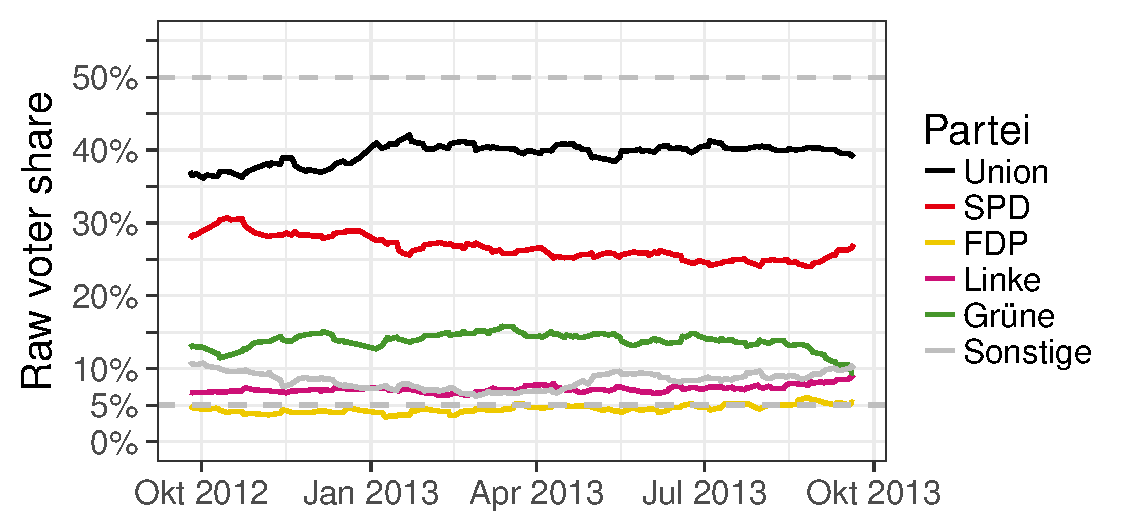
\includegraphics[width=0.6\textwidth]{figures/2013_pooled_rawShares.pdf}
\caption{Course of the pooled party shares from October 2012 until election day on
September 22nd, 2013, based on a pooling time window of 14 days.
As specific voter shares for AfD were only sparsely reported before the election in 2013
the party is contained in ''Others''.
\label{fig:2013}
}
\end{figure}


\paragraph{FDP passing the 5\% hurdle} \ \\
The poll-based prospect of FDP to successfully pass into parliament is visualized
in Figure~\ref{fig:2013_fdp}.
As can be seen, the reported voter share of the party only exceeded the necessary share
of $5\%$ over short periods of time and only once reached a maximum value
of $6\%$ (top left pane in Fig.~\ref{fig:2013_fdp}). Similarly, the probability
for the party to pass the hurdle only rarely rose over $50\%$ (bottom left pane).
However, starting at the end of August 2013 until election day, the pooled voter
shares and the corresponding probabilities consistently lay over $5\%$ and $50\%$,
respectively, stating that -- shortly before election day -- a parliament entry
of the FDP was more probable than not.\\

Comparing voter shares and probabilities, Figure~\ref{fig:2013_fdp} shows
that small changes in the overall share of a party can dramatically influence
event probabilities, depending on the base level of the voter share and
-- in this example -- its closeness to the $5\%$ hurdle.
In this regard, probabilities make it easier to deduce {\it relevant} information
from election polls as they incorporate both the closeness of the observed shares
to the relevant threshold and sample uncertainty.
E.g., the probability corresponding to voter shares of $4\%$ and $6\%$ correspond to
very definite probabilities of near $0\%$ and $100\%$, respectively,
and communicating such probabilities leads to a much clearer perception of
the current public opinion compared to the reported FDP voter share and
survey sample size only.

\begin{figure}[H]\centering
\begin{tabular}{ll}
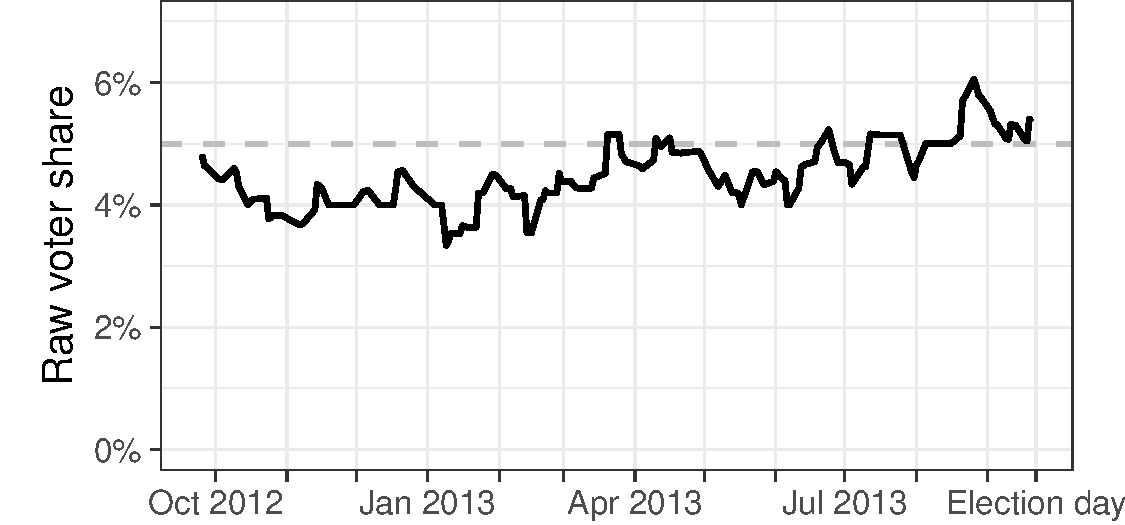
\includegraphics[height=.15\textwidth]{figures/2013_pooled_fdp_rawShares.pdf}
&
\multirow{2}{*}[13ex]{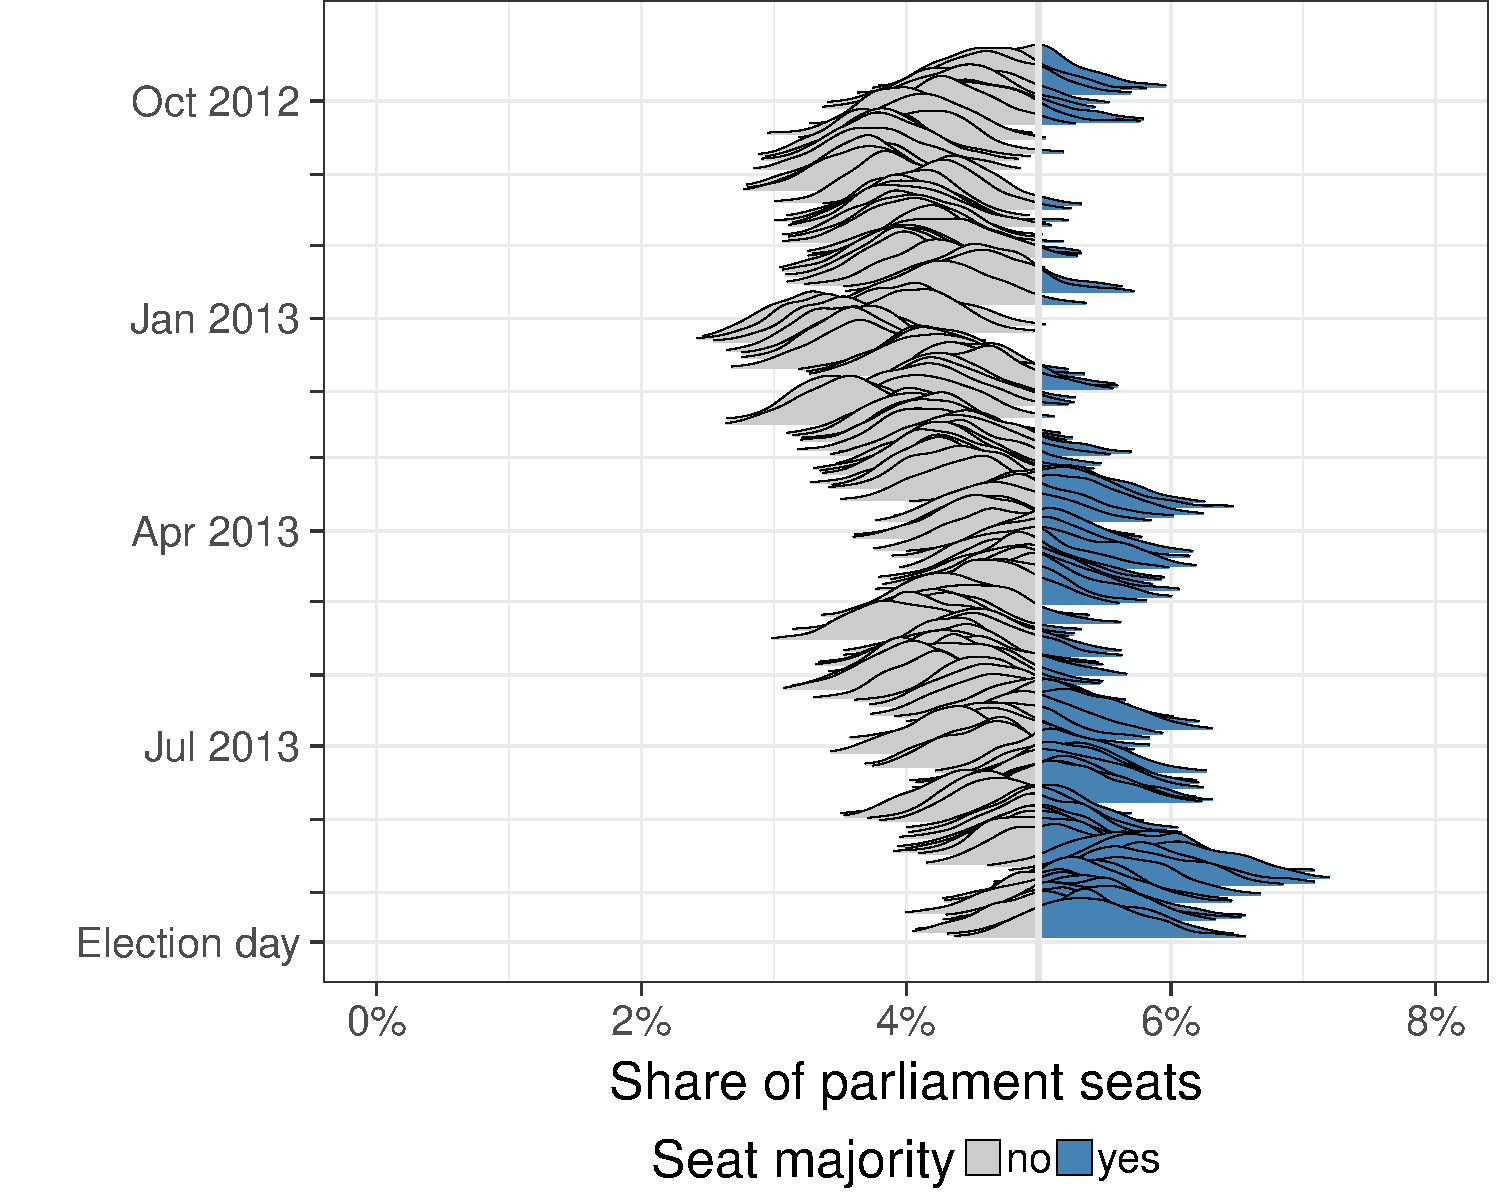
\includegraphics[height=30ex]{figures/2013_pooled_fdp_ridgeline.pdf}}
\\
\includegraphics[height=.15\textwidth]{figures/2013_pooled_fdp_passingProb.pdf}
\end{tabular}
\caption{Development of the prospect of FDP to pass the $5\%$ hurdle before the
German general election in September 2013 based on pooled opinion polls.
Top left: Reported party shares before redistribution. Bottom Left: Probabilities
to pass the $5\%$ hurdle, based on $10\,000$ simulations. Right: Densities of
simulated FDP vote shares based on $10\,000$ simulations over time. Areas under
the density depicted by dark grey indicate the percentage of simulations in which
the FDP would pass the 5\% hurdle.
\label{fig:2013_fdp}
}
\end{figure}


\paragraph{Union-FDP coalition majority} \ \\

Figure \ref{fig:seatDist} shows the simulated
parliament seat shares for the coalition Union-FDP, based on the observed
voter shares in Table \ref{tab_fdp}. The estimated density is clearly bimodal
as the observed FDP share before redistribution equals exactly $5\%$ and
therefore the FDP only enters the parliament in about $50\%$ of the simulations.
In this case, a majority was observed in about one quarter of the simulations,
leading to a estimated event probability of $26\%$.

\begin{figure}[H]\centering
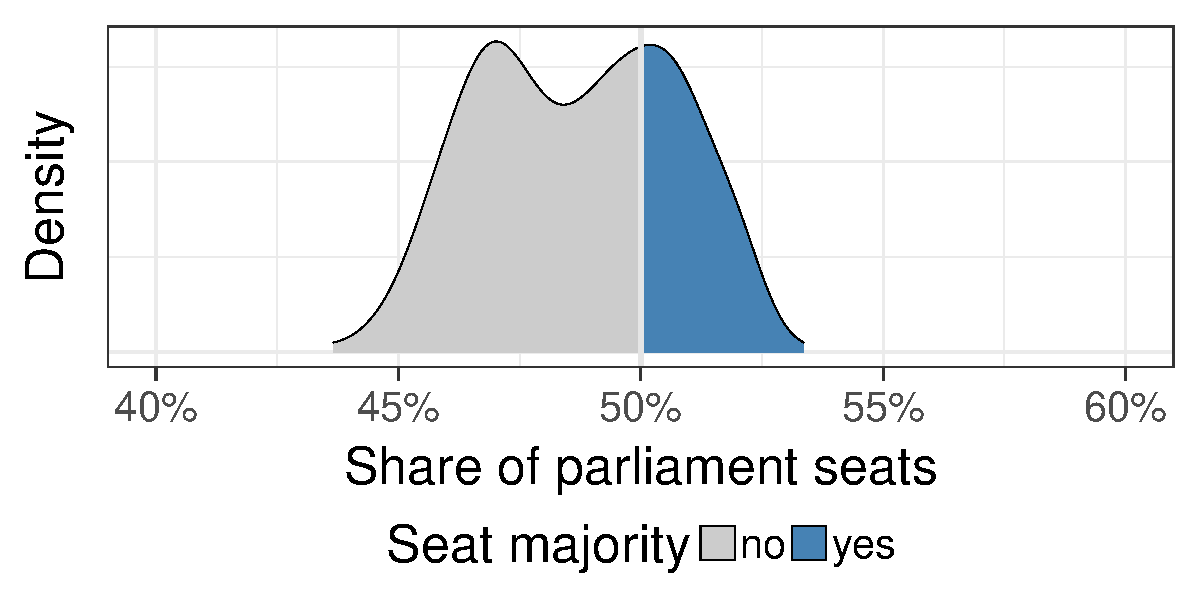
\includegraphics[width=0.45\textwidth]{figures/2013_forsa_cdufdp_lastPreelectionPoll.pdf}
\caption{Density of $10\,000$ simulated parliament seat shares for the coalition
Union-FDP before the German federal election in September 2013 based on the Forsa
opinion poll in Table \ref{tab_fdp}. The area under the density depicted by
dark grey indicates simulations with a Union-FDP majority, resulting in a
probability of about $26\%$.
\label{fig:seatDist}
}
\end{figure}

Such density plots depict both the probability and the underlying
uncertainty for specific events. Therefore they are well suited to communicate
probability estimates as well as the uncertainty underlying opinion polls.
To visualize the {\it development} of such probabilities
for a specific event, e.g., a coalition majority, we recommend extending the
visualization in Figure \ref{fig:seatDist} by using so-called
\emph{ridgeline plots} \citep{wilke_2017} that depict the estimated densities.
In Figure~\ref{fig:seatDist_time} this plot type and the development of majority
probabilities is compared to the joint, redistributed shares of Union-FDP, which
are usually reported in media.

\begin{figure}[H]\centering
\begin{tabular}{ll}
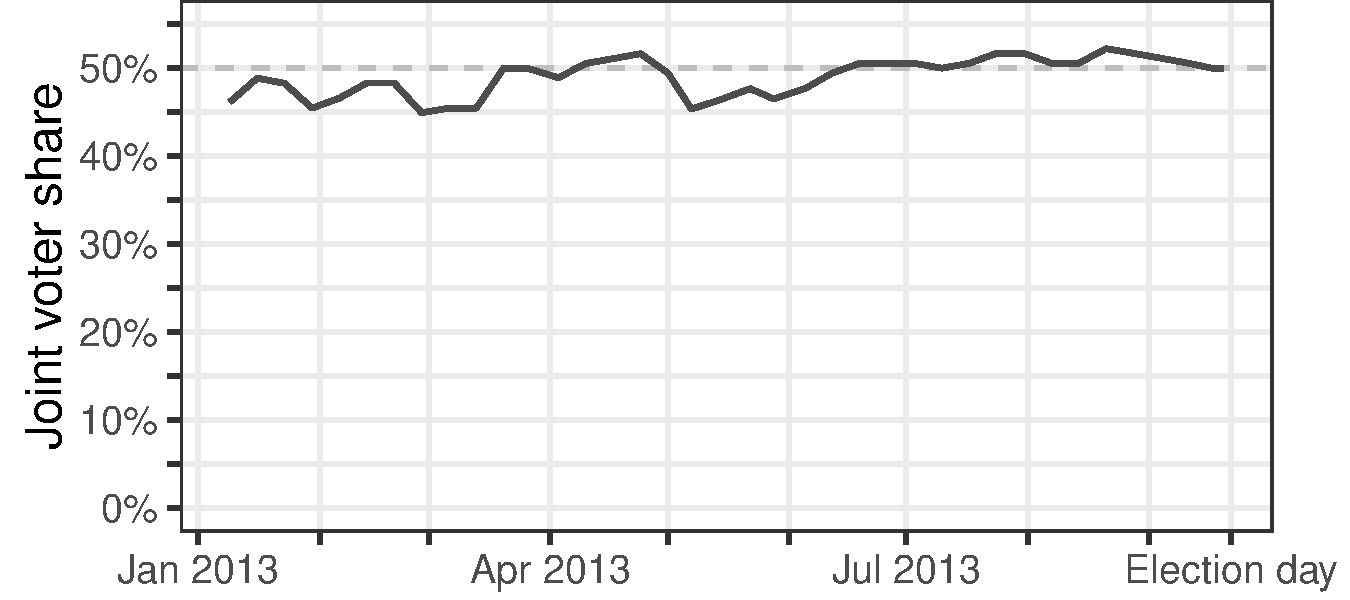
\includegraphics[height=.15\textwidth]{figures/2013_forsa_cdufdp_rawSharesRedist.pdf}
&
\multirow{2}{*}[13ex]{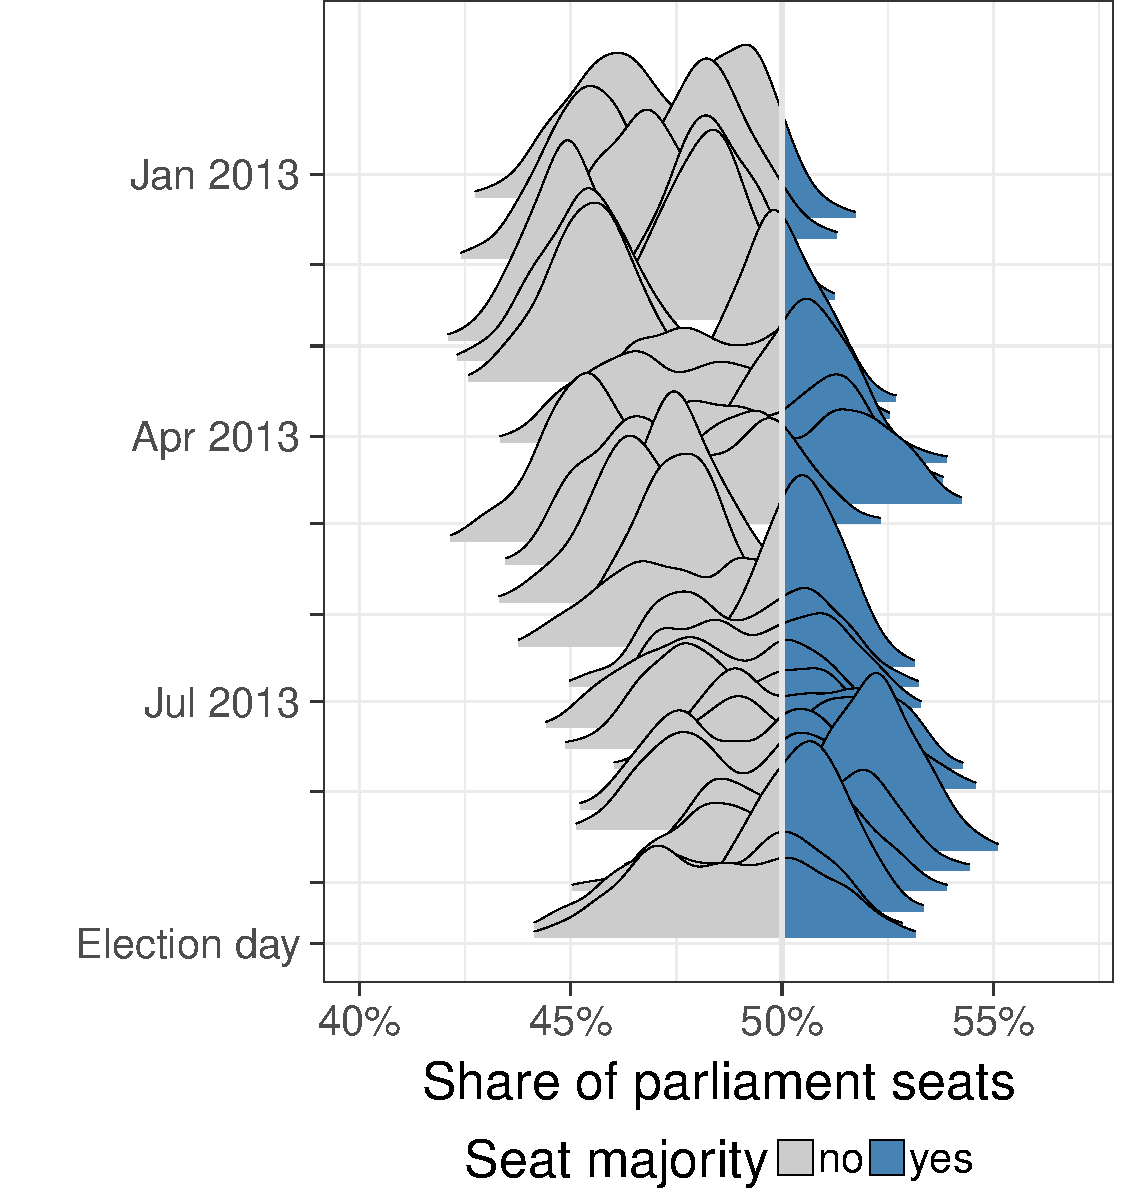
\includegraphics[height=30ex]{figures/2013_forsa_cdufdp_ridgeline.pdf}}
\\
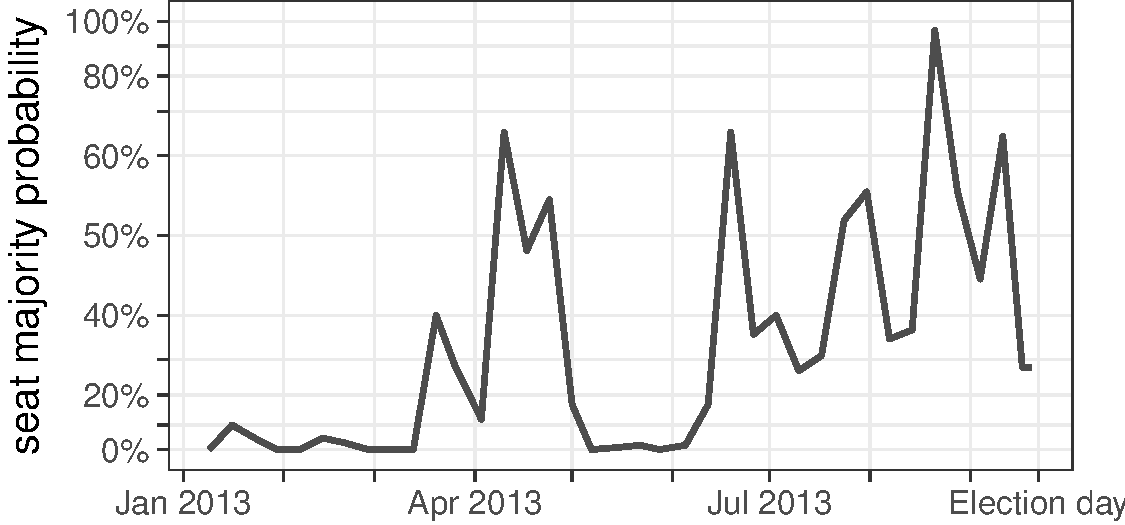
\includegraphics[height=.15\textwidth]{figures/2013_forsa_cdufdp_prob.pdf}
\end{tabular}
\caption{Development of the prospect for the coalition Union-FDP to form a
government majority before the German general election in September 2013 based on
Forsa opinion polls.
Top left: Reported joint voter shares for Union-FDP after redistribution.
Bottom left: Probabilities to reach a majority of seats in parliament, based on
$10\,000$ simulations from the posterior.
Right: Densities of simulated parliament seat shares based on $10\,000$ simulations.
The area under the density depicted by dark grey indicates simulations with a
Union-FDP majority.
\label{fig:seatDist_time}
}
\end{figure}

Comparing the redistributed voter shares and the seat majority probabilities
in Figure~\ref{fig:seatDist_time} it is clear that the probabilities contain
a lot more information than the voter shares. Especially, even small changes
in the redistributed voter share can make an immense difference regarding the
probability of the coalition to form a government.\\

To focus on the most relevant changes in the majority probabilities, we propose
the use of a skewed axis as shown in Figure~\ref{fig:seatDist_time}. In this axis
the range of values around $50\%$ is stretched and the range of values near
$0\%$ and $100\%$ is compressed (MORE details needed, what is the exact transformation?).
In this way, we put less weight on changes
where an event is {\it still highly (im)probable} and emphasize more relevant
changes after which an event gets more or less probable than $50\%$. Also,
consistently using another axis for the estimated probabilities prevents
confusion of probabilities and voter shares.\\

Finally, Figure \ref{fig:2013_cdufdp} visualizes the results for the potential
coalition Union-FDP based on \emph{pooled} opinion polls (cf. Section \ref{ssec:pooling}).
The redistributed, joint voter share was around $43\%$ in October 2012,
and rose steadily over time, reaching its maximum of ca. $51\%$ about one month
before election day.
Only taking this development of the redistributed voter shares into
consideration, one would conclude that -- apart from a short
time window in August/September of 2013 -- a majority of the Union-FDP
coalition would be slightly missed.
In the best case, sample uncertainty would be reported, making
a majority for the coalition {\it (highly) improbable}. A more
precise and adequate quantification of the uncertainty however is usually not given.

\begin{figure}[H]\centering
\begin{tabular}{ll}
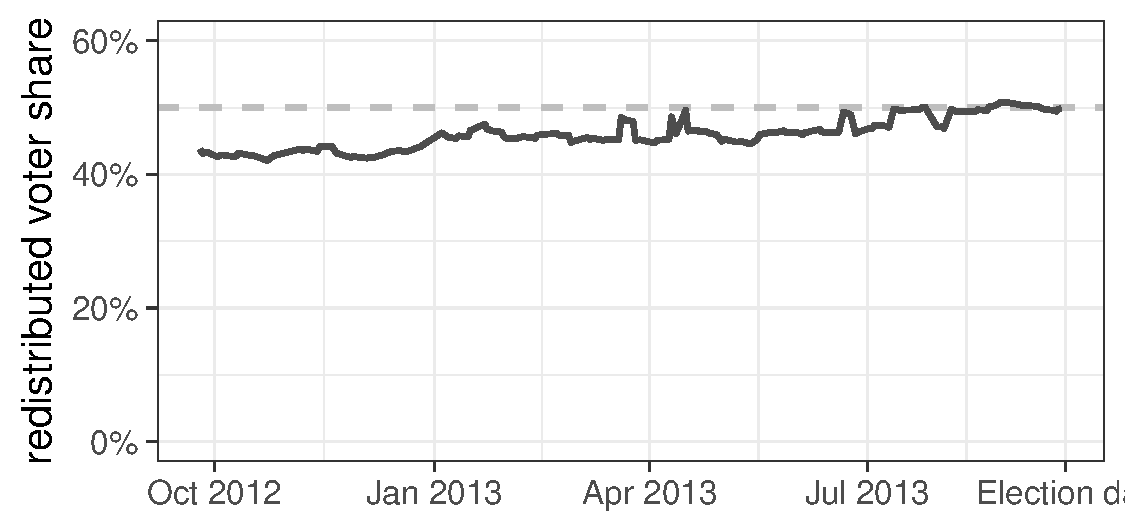
\includegraphics[height=.15\textwidth]{figures/2013_pooled_cdufdp_rawSharesRedist.pdf}
&
\multirow{2}{*}[13ex]{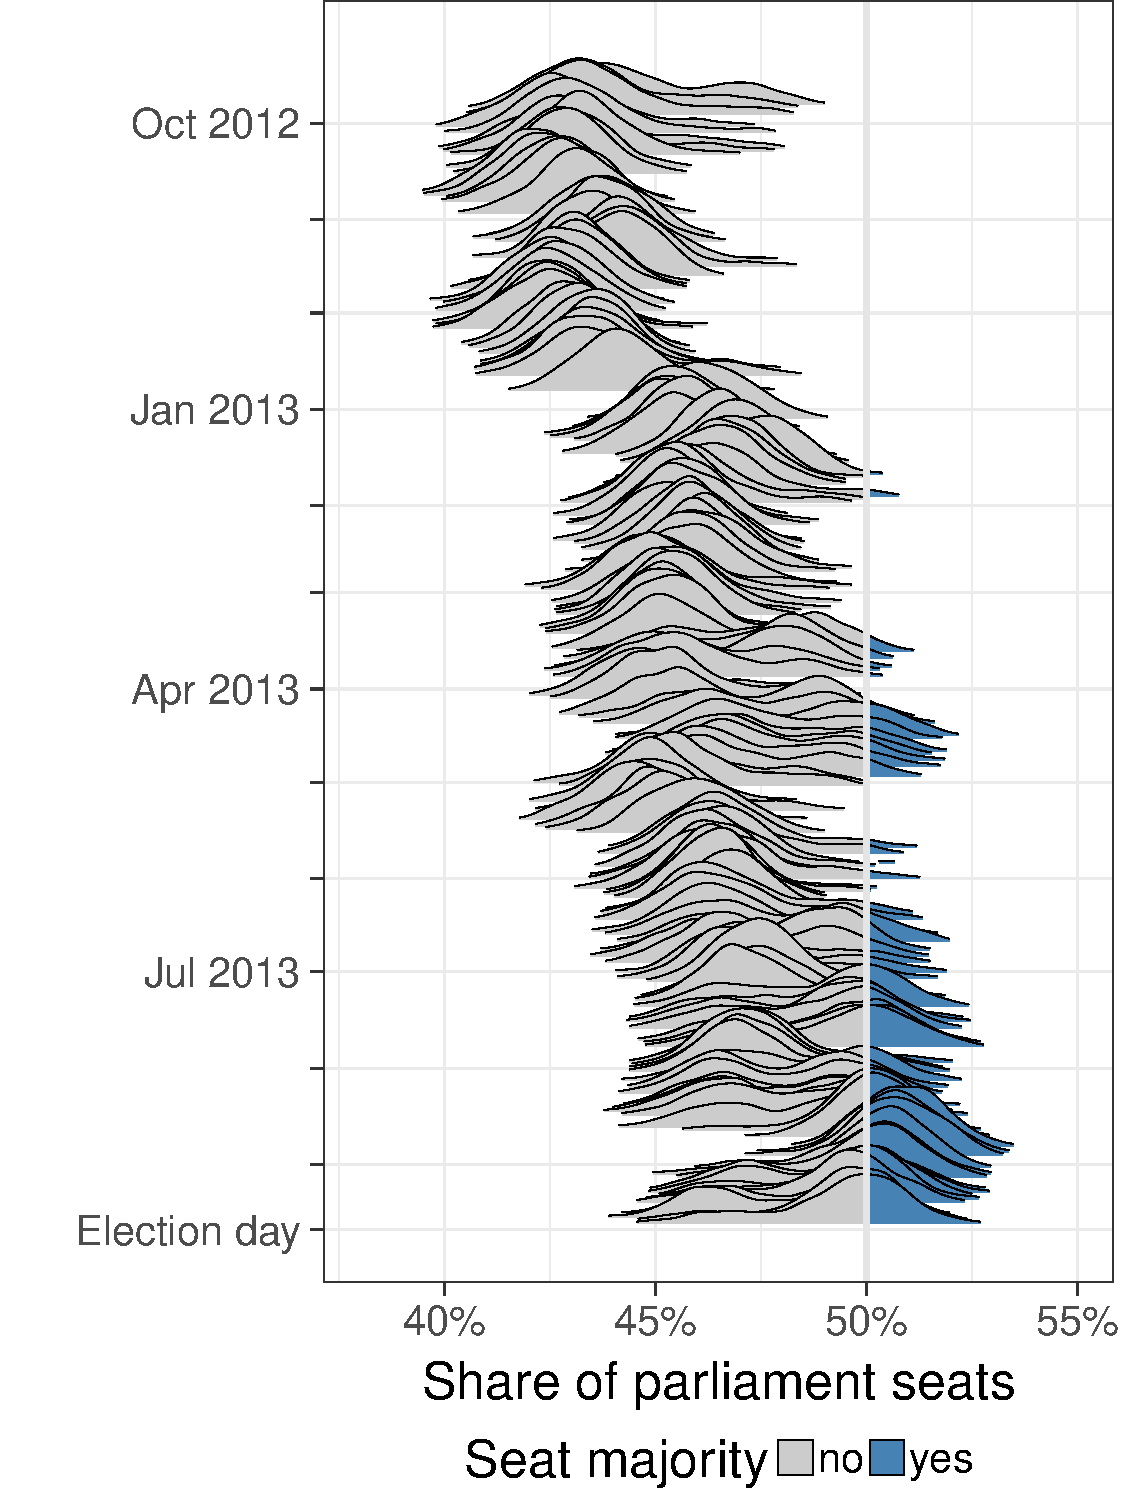
\includegraphics[height=.3\textwidth]{figures/2013_pooled_cdufdp_ridgeline.pdf}}
\\
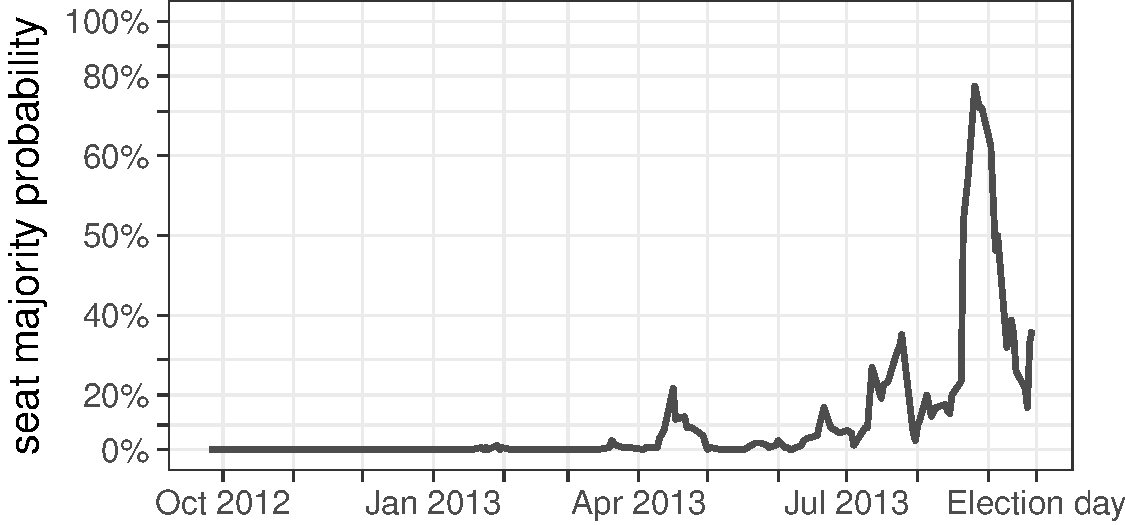
\includegraphics[height=.15\textwidth]{figures/2013_pooled_cdufdp_prob.pdf}
\end{tabular}
\caption{Development of the prospect that the coalition Union-FDP would obtain
the majority of parliament seats before the German general election in September
2013 based on \emph{pooled} opinion polls. Top: Observed joint voter shares after
redistribution. Bottom: Probabilities to obtain the majority of parliament seats,
based on $10\,000$ simulations.
Right: Densities of simulated parliament seat shares based on $10\,000$ simulations.
Areas under the density depicted by dark grey indicate the percentage of
simulations with a seat majority for Union-FDP.
\label{fig:2013_cdufdp}
}
\end{figure}

Considering the estimated seat majority probabilities together with
the simulated seat share densities instead draws a more comprehensive picture
of the situation.
While the overall development of probabilities has the same structure
as the redistributed voter shares, i.e., increase over time with time,
there are two points that clearly get more weight when shifting
the focus in reporting towards discussing {\it how probable} events are:
First of all, the impact of small changes in voter shares is more pronounced
in the probability development. As discussed in context of
Figure~\ref{fig:2013_fdp}, the effect of changes in voter shares on
probabilities of an event strongly depends on the base level of the voter shares.
For example, a rise in voter shares from $45\%$ to $48\%$ in March 2013 only had a
very small impact on the event probabilities, as a seat majority was still very improbable.
Instead, even very small changes near a voter share of $50\%$ heavily influence
the event probabilities. Secondly, probabilities do not only take into account
the joint party shares and the sample uncertainty,
but also implicitly cover the uncertainty regarding whether FDP passes the $5\%$
hurdle or not. Apart from the end of August 2013, the latter event
is highly uncertain and thus overall majority probabilities of
the coalition are comparatively small, even for pooled voter shares around $50\%$.
The impact of the uncertainty regarding the FDP entering the parliament is
directly noticeable in the ridgeline plot (right panel in Fig.~\ref{fig:2013_cdufdp}),
as the densities are bimodal or unimodal depending on whether the reported FDP
share is close to $5\%$ or not (see Fig.~\ref{fig:2013_fdp}), respectively.



\subsection{German federal election 2017} \label{subsec:2017}
After the federal election in 2013, none of the desired coalitions
reached a seat majority and a "grand coalition" between Union and the social
democratic SPD formed the government from 2013 to 2017.
For the following election on September 24th, 2017, the goal of both Union and SPD
was to obtain enough votes to form a governance coalition outside the grand
coalition. Therefore, multiple potential coalitions were of interest before the
election. In the following paragraphs, we will focus on the most prominently
discussed coalitions, i.e., the Union-led coalition Union-FDP, and the
SPD-led coalition of SPD, the Left party (Die LINKE) and the Green party, which
-- based on the joint voter share -- was the strongest alternative to a Union-led
government and was not clearly denied by the member parties until several weeks
before election day.
Also, after the rise of the right-wing party AfD major interest was
in whether this party, which slightly missed the $5\%$ hurdle in 2013,
would become the third strongest party in parliament after Union and SPD.
The pooled party shares before the 2017 election are shown in Figure~\ref{fig:2017}.

\begin{figure}[H]\centering
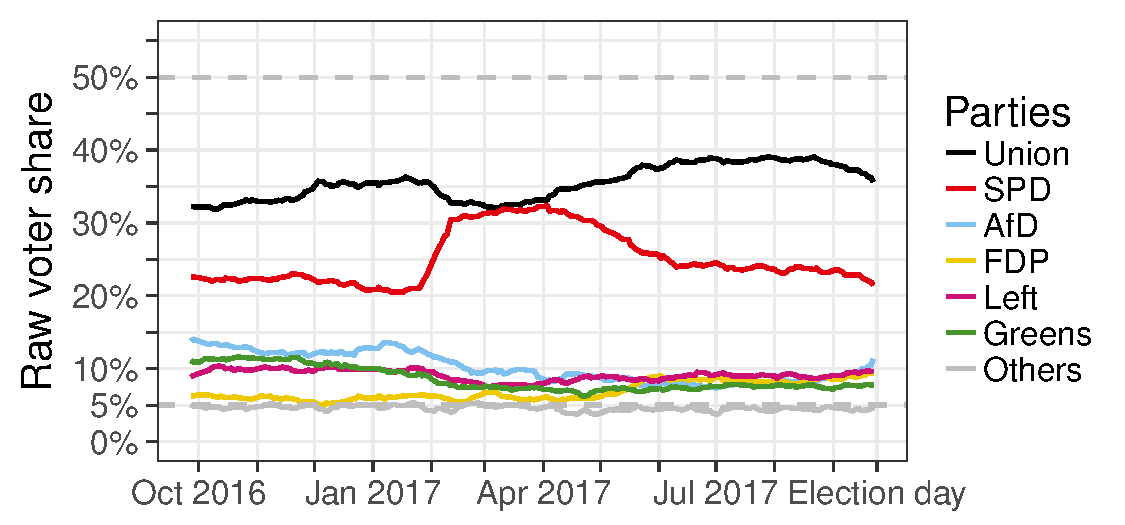
\includegraphics[width=0.6\textwidth]{figures/2017_pooled_rawShares.pdf}
\caption{Development of the pooled raw voter shares from October 2016 until
election day on September 24, 2017, based on a pooling time window of 14 days.
\label{fig:2017}
}
\end{figure}


\paragraph{Union-FDP coalition majority} \ \\
Compared to the federal election 2013, the situation for a
coalition between Union and FDP before the election in 2017
was quite different as FDP voter shares were
clearly above the $5\%$ hurdle (see Fig.~\ref{fig:2017}) most of the time.
However, as the share of Union was lower than in 2013,
the joint redistributed voter share was mostly below $50\%$.
As can be seen in Figure~\ref{fig:2017_cdufdp}, the coalition had
a joint, redistributed share of about $40\%$ in October 2016
and reached its maximum share of nearly $49.8\%$ about one month
before election day.

Again, interpreting only the observed redistributed voter shares
is hard for the general public as no easily accessible quantification
of uncertainty is given. By comparison, the ridgeline plot in Figure~\ref{fig:2017_cdufdp}
shows that parliament seat shares (or correspondingly voter shares)
below $48\%$ correspond to negligibly small success probabilities
of $<1\%$, based on pooled effective sample sizes of around $3000$.
On the other hand, based on comparable sample sizes, observed shares of $49\%$
and $49.5\%$ corresponded to probabilities of around $14\%$ and $25\%$,
respectively.

Overall, one month before election day the coalition had a good prospect
reaching a seat majority based on a redistributed share of $49.8\%$ and
a probability of nearly $40\%$.
However, until two days before the election the pooled share and the probability
dropped again to $47.4\%$ and $0.4\%$, respectively, making a success
of the two parties highly improbable.

\begin{figure}[H]\centering
\begin{tabular}{ll}
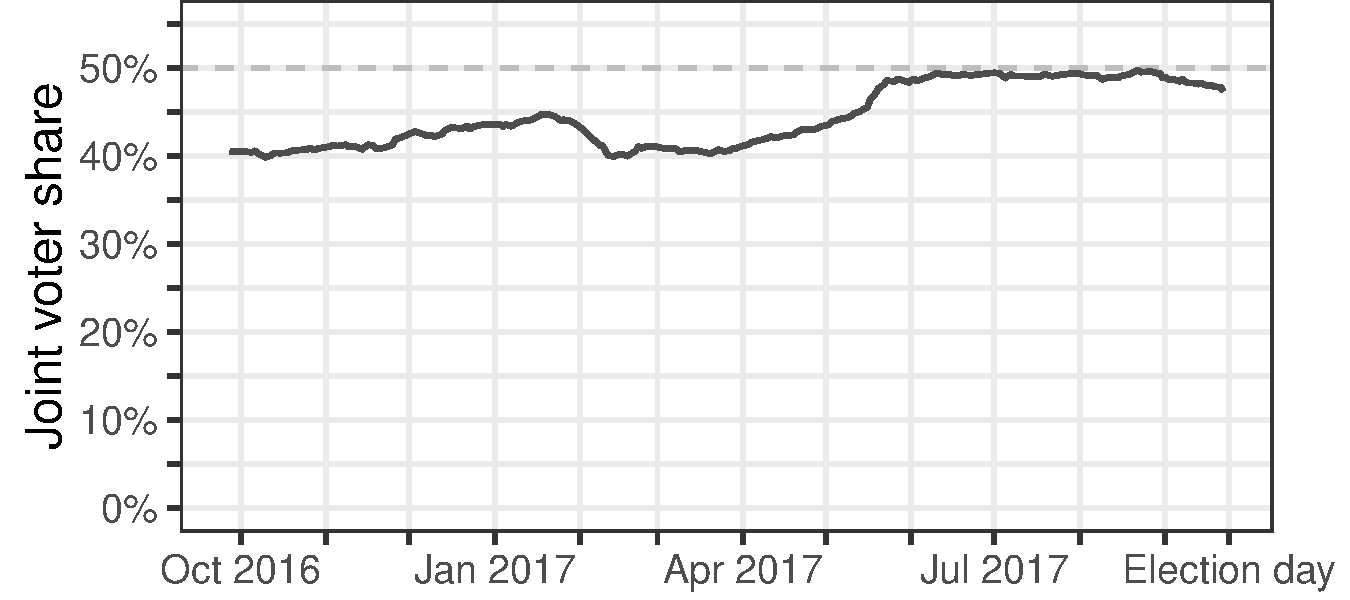
\includegraphics[height=.15\textwidth]{figures/2017_pooled_cdufdp_rawSharesRedist.pdf}
&
\multirow{2}{*}[13ex]{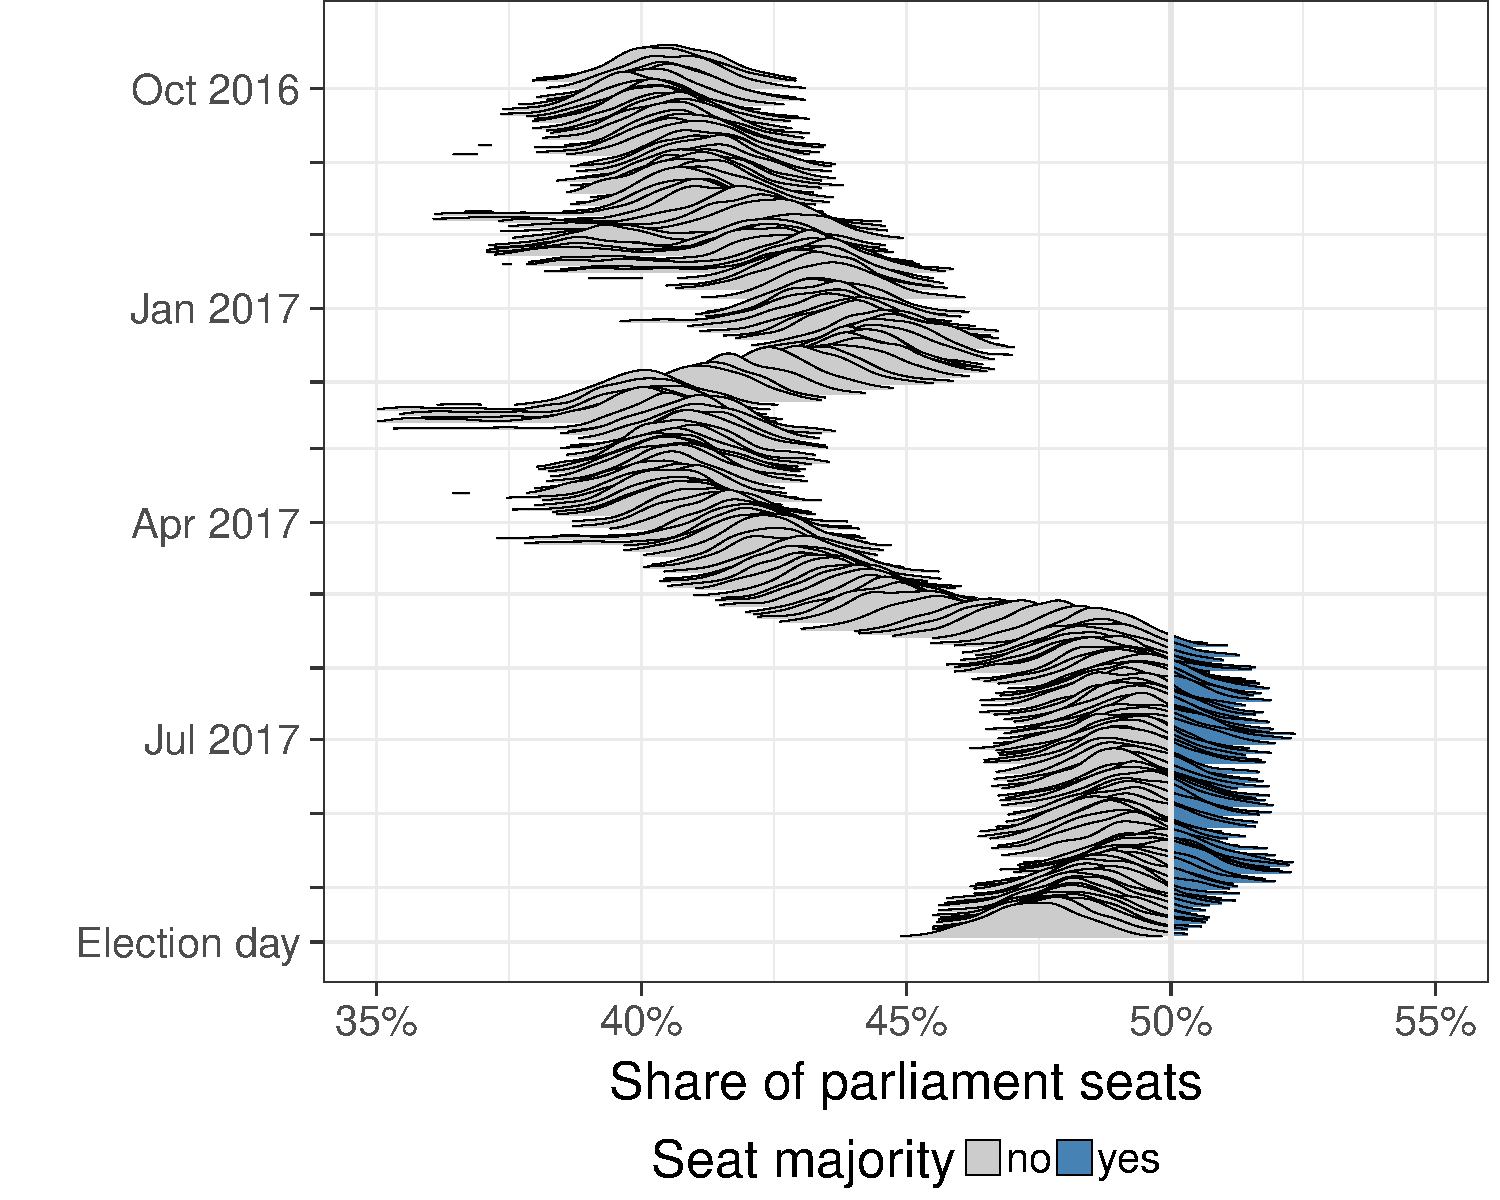
\includegraphics[height=30ex]{figures/2017_pooled_cdufdp_ridgeline.pdf}}
\\
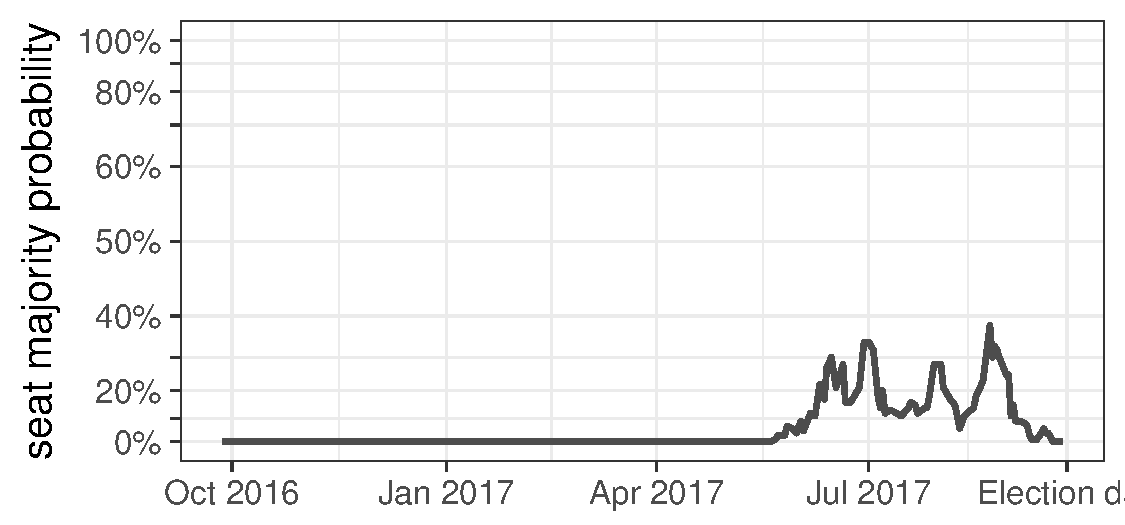
\includegraphics[height=.15\textwidth]{figures/2017_pooled_cdufdp_prob.pdf}
\end{tabular}
\caption{Development of the prospect to form a government of the coalition
Union-FDP before the German general election in September 2017 based on pooled
opinion polls.
Top left: Reported voter shares after redistribution.
Bottom left: Probabilities to reach a majority of seats in parliament, based on
$10\,000$ simulations.
Right: Densities of simulated parliament seat shares based on $10\,000$ simulations.
The area under the density depicted by dark grey indicates simulations with a
Union-FDP majority.
\label{fig:2017_cdufdp}
}
\end{figure}


\paragraph{SPD-Left-Greens coalition majority} \ \\
Regarding the party share development of the SPD, the year before
the general election in 2017 was shaped by an unusually fast increase, starting
at the end of January 2017, when Martin Schulz was elected to be the SPD chancellor
candidate and a subsequent, steady decline from April 2017 on (see Fig.~\ref{fig:2017}).
Accordingly, the coalition between SPD, the Left and the Greens had
their best joint poll results between February and May 2017 as is shown in
Figure~\ref{fig:2017_spdleftgreens}.
The maximum share was reached in April with a redistributed voter
share of $\sim 50\%$, which corresponded to a probability of obtaining the
parliament seat majority of $\sim 48\%$.
Starting in April, the probability again dropped to negligibly small values.
Shortly before election day, the joint share
reached a value of around $41\%$ and event probabilities of practically zero.
The ridgeline plot in Figure~\ref{fig:2017_spdleftgreens}
again nicely visualizes the uncertainty underlying the event of
interest. This is not only limited to parties forming the potential coalition,
but also includes information about all other causes of uncertainty in the data.
For example, in November and December of 2016, the seat share distribution clearly
is bimodal as in a relevant share of simulations FDP does not pass
the $5\%$ hurdle and more votes are redistributed in these cases.

\begin{figure}[H]\centering
\begin{tabular}{ll}
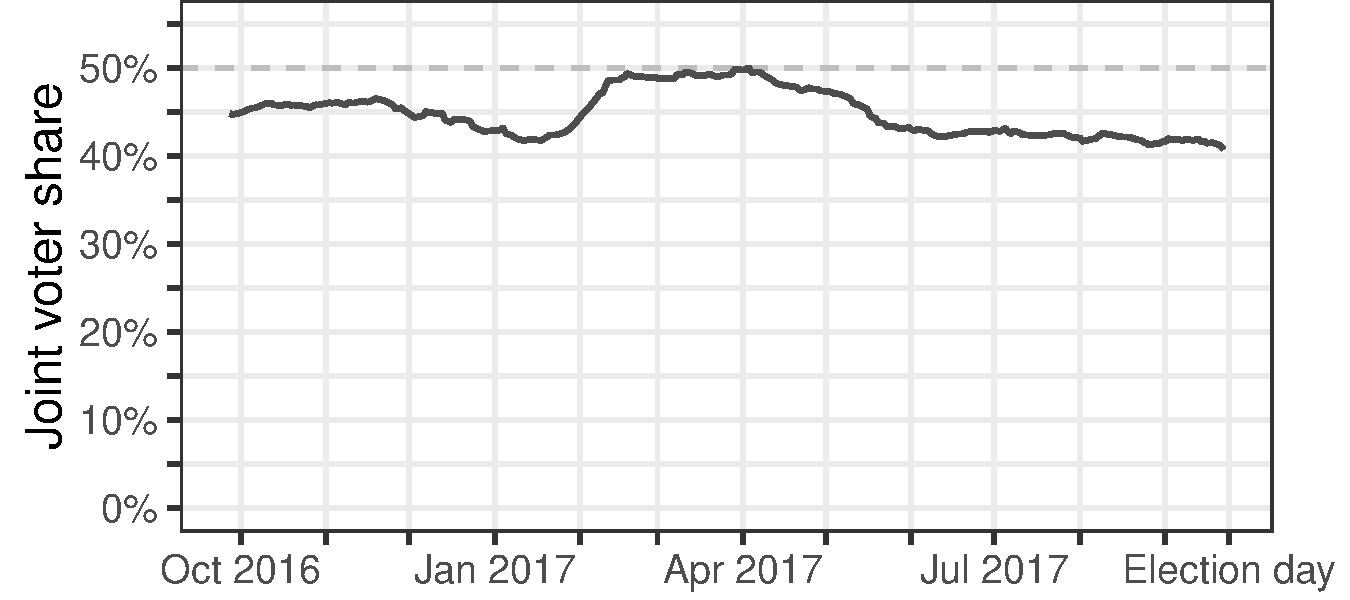
\includegraphics[height=.15\textwidth]{figures/2017_pooled_spdleftgreens_rawSharesRedist.pdf}
&
\multirow{2}{*}[13ex]{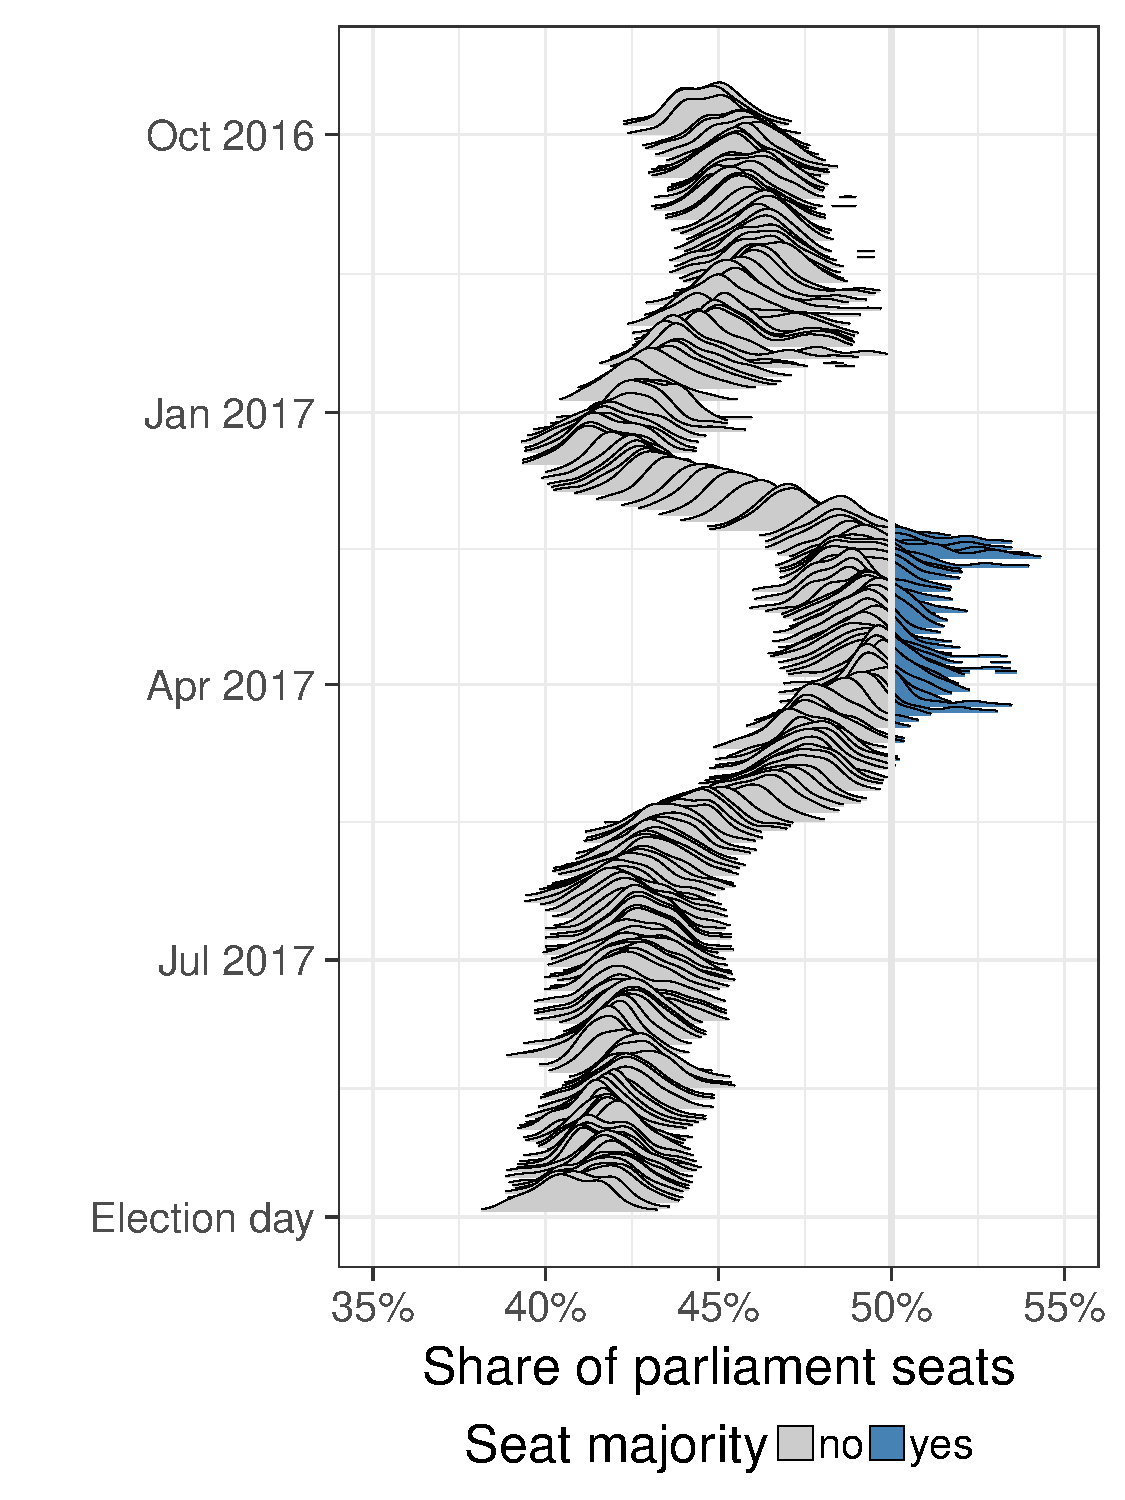
\includegraphics[height=30ex]{figures/2017_pooled_spdleftgreens_ridgeline.pdf}}
\\
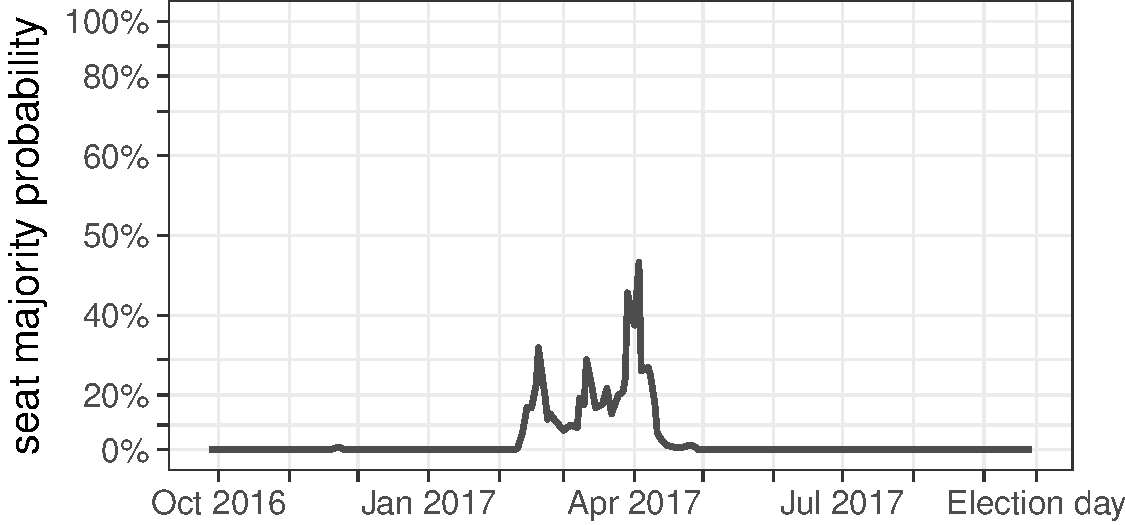
\includegraphics[height=.15\textwidth]{figures/2017_pooled_spdleftgreens_prob.pdf}
\end{tabular}
\caption{Development of the prospect that the coalition SPD-Left-Greens will
obtain a majority of parliament seats before the German
general election in September 2017, based on pooled opinion polls.
Top left: Observed voter shares after redistribution.
Bottom left: Probabilities to obtain a seat majority based on $10\,000$ simulations.
Right: Densities of simulated parliament seat shares based on $10\,000$ simulations.
The area under the density depicted by dark grey indicates simulations with a
seat majority.
\label{fig:2017_spdleftgreens}
}
\end{figure}


\paragraph{AfD becoming third strongest party} \ \\
In the pretext to the 2017 election, special interest was given to the question
which party would the third largest party in parliament.
With observed voter shares of over $8\%$, the right-wing AfD had a very good
prospect to become a member of the German parliament for the first time
(see Fig.~\ref{fig:2017_afd}) and was polling close to other opposition parties.
Using our KOALA approach, estimating probabilities for the event that AfD becomes
third largest party in parliament is straight forward, adequately summarizing
this event probability that simultaneously depends on all reported party shares.

In the year before the general election in 2017, reported AFD party shares
underwent strong fluctuations. In January 2017 the party had a $3.9\%$ lead
over Left and Greens (corresponding to an estimated probability of becoming the
third largest party in parliament of $100\%$). Subsequently, the AfD share
dropped $1.9$ percentage points behind the Left in June
(corresponding to a $1.2\%$ probability)
and rose back to a $1.7$ percentage point lead (in voter shares) lead over the Left
and FDP shortly before election day (corresponding to a $96.8\%$ event probability).

\begin{figure}[H]\centering
\begin{tabular}{l}
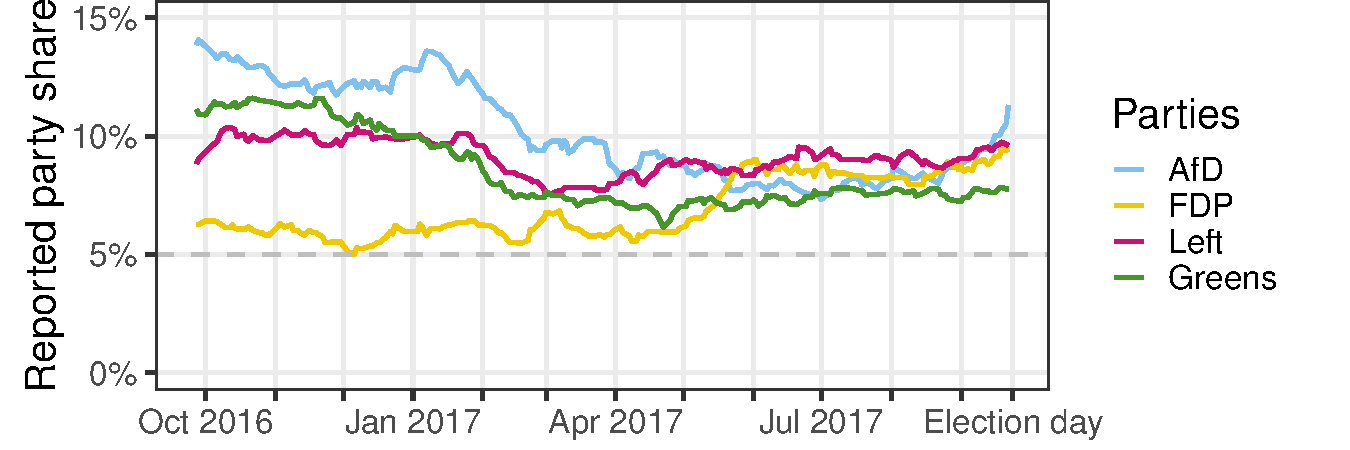
\includegraphics[height=.2\textwidth]{figures/2017_pooled_afd_rawShares.pdf}
\\
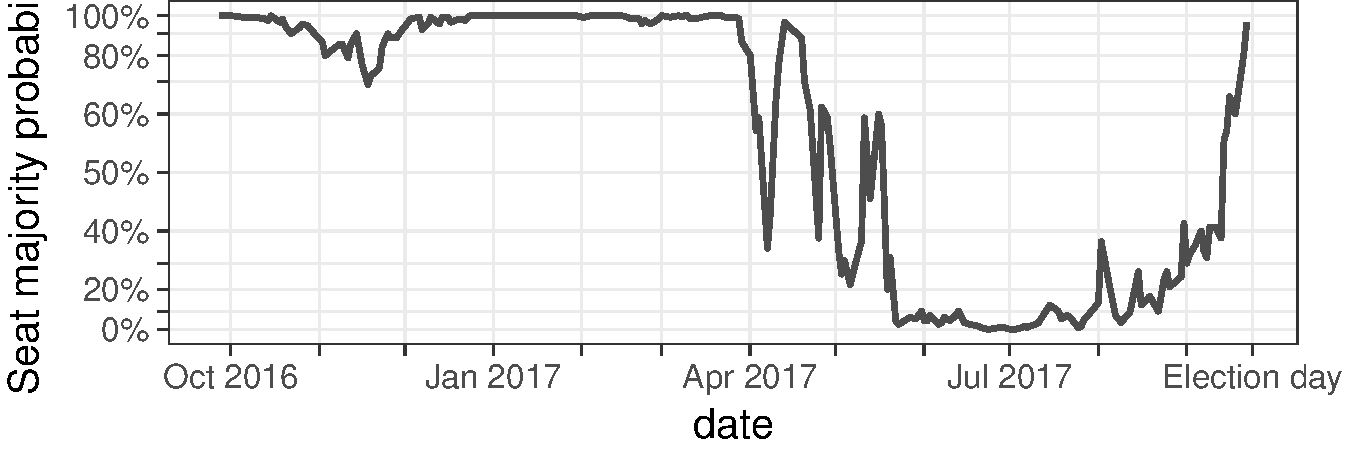
\includegraphics[height=.15\textwidth]{figures/2017_pooled_afd_thirdPartyProb.pdf}
\end{tabular}
\caption{Development of the prospect that AfD becomes the third largest party
in parliament before the German general election in September 2017 based on pooled
opinion polls.
Top: Observed voter shares before redistribution.
Bottom: Probabilities to become third strongest party, based on $10\,000$ simulations.
\label{fig:2017_afd}
}
\end{figure}


\section{Conclusion} \label{sec:conclusion}
We presented the KOALA (Coalition analysis) approach,
i.e. a Bayesian, Monte Carlo based method to estimate probabilities of specific
election outcomes based on publicly available opinion polls.
A pooling approach allows for the inclusion of information from multiple
surveys and reduces sample uncertainty.
The estimated event probabilities are easy to communicate to the general
public and prevent improper poll-based reporting as they include
sample uncertainty in a natural way.
We visualize the results on a publicly available website for chosen elections and
provide the open-source \texttt{R} package \texttt{coalitions} that allows for a
straightforward application of the method to any multi-party electoral system.
In this manner, our long-term goal is to make proper uncertainty assessment
in general opinion poll-based reporting the rule, rather than an exception.



% % For one-column wide figures use
% \begin{figure}
% % Use the relevant command to insert your figure file.
% % For example, with the graphicx package use
%   \includegraphics{figures/seatDist_ridgeline.pdf}
% % figure caption is below the figure
% \caption{Please write your figure caption here}
% \label{fig:1}       % Give a unique label
% \end{figure}
% %
% % For two-column wide figures use
% \begin{figure*}
% % Use the relevant command to insert your figure file.
% % For example, with the graphicx package use
%   \includegraphics[width=0.75\textwidth]{figures/seatDist_ridgeline.pdf}
% % figure caption is below the figure
% \caption{Please write your figure caption here}
% \label{fig:2}       % Give a unique label
% \end{figure*}
%
% % For tables use
% \begin{table}
% % table caption is above the table
% \caption{Please write your table caption here}
% \label{tab:1}       % Give a unique label
% % For LaTeX tables use
% \begin{tabular}{lll}
% \hline\noalign{\smallskip}
% first & second & third  \\
% \noalign{\smallskip}\hline\noalign{\smallskip}
% number & number & number \\
% number & number & number \\
% \noalign{\smallskip}\hline
% \end{tabular}
% \end{table}


%\begin{acknowledgements}
%If you'd like to thank anyone, place your comments here
%and remove the percent signs.
%\end{acknowledgements}

% BibTeX users please use one of
% \bibliographystyle{spbasic}      % basic style, author-year citations
%\bibliographystyle{spmpsci}      % mathematics and physical sciences
%\bibliographystyle{spphys}       % APS-like style for physics
\bibliography{bauer_2018}   % name your BibTeX data base

% Non-BibTeX users please use
% \begin{thebibliography}{}
%
% and use \bibitem to create references. Consult the Instructions
% for authors for reference list style.
%
% \bibitem{RefJ}
% % Format for Journal Reference
% Author, Article title, Journal, Volume, page numbers (year)
% % Format for books
% \bibitem{RefB}
% Author, Book title, page numbers. Publisher, place (year)
% % etc
% \end{thebibliography}

\end{document}
% end of file template.tex
